\documentclass{article}
\usepackage[utf8x]{inputenc}
\usepackage{ucs}
\usepackage{amsmath} 
\usepackage{amsfonts}
\usepackage{marvosym}
\usepackage{wasysym}
\usepackage{upgreek}
\usepackage[english,russian]{babel}
\usepackage{graphicx}
\usepackage{float}
\usepackage{textcomp}
\usepackage{hyperref}
\usepackage{geometry}
  \geometry{left=2cm}
  \geometry{right=1.5cm}
  \geometry{top=1cm}
  \geometry{bottom=2cm}
\usepackage{tikz}
\usepackage{ccaption}
\usepackage{multicol}

\hypersetup{
   colorlinks=true,
   citecolor=blue,
   linkcolor=black,
   urlcolor=blue
}

\usepackage{listings}
%\setlength{\columnsep}{1.5cm}
%\setlength{\columnseprule}{0.2pt}

\usepackage[absolute]{textpos}


\usepackage{colortbl,graphicx,tikz}
\definecolor{X}{rgb}{.5,.5,.5}

\renewcommand{\thesubsection}{\arabic{subsection}}

\begin{document}
\pagenumbering{gobble}
\lstset{
  language=C++,                % choose the language of the code
  basicstyle=\linespread{1.1}\ttfamily,
  columns=fixed,
  fontadjust=true,
  basewidth=0.5em,
  keywordstyle=\color{blue}\bfseries,
  commentstyle=\color{gray},
  stringstyle=\ttfamily\color{orange!50!black},
  showstringspaces=false,
  numbersep=5pt,
  numberstyle=\tiny\color{black},
  numberfirstline=true,
  stepnumber=1,                   % the step between two line-numbers.        
  numbersep=10pt,                  % how far the line-numbers are from the code
  backgroundcolor=\color{white},  % choose the background color. You must add \usepackage{color}
  showstringspaces=false,         % underline spaces within strings
  captionpos=b,                   % sets the caption-position to bottom
  breaklines=true,                % sets automatic line breaking
  breakatwhitespace=true,         % sets if automatic breaks should only happen at whitespace
  xleftmargin=.2in,
  extendedchars=\true,
  keepspaces = true,
}
\lstset{literate=%
   *{0}{{{\color{red!20!violet}0}}}1
    {1}{{{\color{red!20!violet}1}}}1
    {2}{{{\color{red!20!violet}2}}}1
    {3}{{{\color{red!20!violet}3}}}1
    {4}{{{\color{red!20!violet}4}}}1
    {5}{{{\color{red!20!violet}5}}}1
    {6}{{{\color{red!20!violet}6}}}1
    {7}{{{\color{red!20!violet}7}}}1
    {8}{{{\color{red!20!violet}8}}}1
    {9}{{{\color{red!20!violet}9}}}1
}
\newcommand\upquote[1]{\textquotesingle#1\textquotesingle}

\renewcommand{\thesubsection}{\arabic{subsection}}
\makeatletter
\def\@seccntformat#1{\@ifundefined{#1@cntformat}%
   {\csname the#1\endcsname\quad}%    default
   {\csname #1@cntformat\endcsname}}% enable individual control
\newcommand\section@cntformat{}     % section level 
\newcommand\subsection@cntformat{Задача \thesubsection.\space} % subsection level
\newcommand\subsubsection@cntformat{\thesubsubsection.\space} % subsubsection level
\makeatother


\makeatletter
\newcount\my@repeat@count
\newcommand{\myrepeat}[2]{%
  \begingroup
  \my@repeat@count=\z@
  \@whilenum\my@repeat@count<#1\do{#2\advance\my@repeat@count\@ne}%
  \endgroup
}
\makeatother

\title{Семинар \#1: Потоки. Домашнее задание.\vspace{-5ex}}\date{}\maketitle

\subsection{Запуск \texttt{n} потоков}
Напишите программу, которая будет считывать целое число \texttt{n} из стандартного входа и создавать \texttt{n} новых потоков. \texttt{i}-й поток должен делать следующее:
\begin{itemize}
\item Писать сообщение: "Thread \#i started."
\item Ждать \texttt{i} секунд
\item Писать сообщение: "Thread \#i finished."
\end{itemize}

Для ожидания используйте функцию \texttt{sleep\_for} из пространства имён \texttt{std::this\_thread}. Пример использования этой функции:
\begin{lstlisting}
#include <iostream>
#include <thread>
#include <chrono>
using namespace std::chrono_literals;

int main()
{
    std::this_thread::sleep_for(1s);
    std::cout << "Waited for 1 second" << std::endl;
    
    std::this_thread::sleep_for(100ms);
    std::cout << "Waited for 100 millisecond" << std::endl;
}
\end{lstlisting}

\begin{center}
\includegraphics[scale=1]{../images/n_threads.png}
\end{center}

\subsection{Запуск потока в потоке}
Напишите программу, которая будет считывать целое число \texttt{n} из стандартного входа и создавать \texttt{n} потоков. Но при этом главный поток (функция \texttt{main}) должен создать только первый поток. Второй поток должен создасться внутри первого. Третий -- внутри второго. И так далее. Вообщем \texttt{i}-й поток должен:
\begin{itemize}
\item Писать сообщение: "Thread \#i started."
\item Ждать \texttt{200} миллисекунд
\item Создавать \texttt{(i+1)}-й поток.
\item Дожидаться завершения \texttt{(i+1)}-го потока с помощью метода \texttt{join}.
\item Ждать \texttt{200} миллисекунд
\item Писать сообщение: "Thread \#i finished."
\end{itemize}

\begin{center}
\includegraphics[scale=1]{../images/n_threads_mat.png}
\end{center}


\subsection{Поиск максимума}
В файле \texttt{code/00problem\_paralel\_max.cpp} написана функция:
\begin{lstlisting}
uint64_t getMax(const std::vector<uint64_t>& v)
\end{lstlisting}
которая принимает вектор чисел и возвращает максимальный элемент в этом векторе.
Напишите функцию:
\begin{lstlisting}
uint64_t getMax(int n, const std::vector<uint64_t>& v)
\end{lstlisting}
которая будет делать то же самое, но параллельно, используя \texttt{n} потоков.
Протестируйте функцию, замерив скорость работы однопоточной и многопоточной версии.


\subsection{Поиск максимума на диапазоне}
В файле \texttt{code/01problem\_paralel\_max\_iterators.cpp} написана шаблонная функция:
\begin{lstlisting}
template <typename RandIt>
RandIt getMax(RandIt start, RandIt finish)
\end{lstlisting}
которая принимает два random-access итератора и находит максимальный элемент на диапазоне, задаваемом этими итераторами. Функция возвращает итератор на максимальный элемент.
Напишите шаблонную функцию:
\begin{lstlisting}
template <typename RandIt>
RandIt getMax(int n, RandIt start, RandIt finish)
\end{lstlisting}
которая будет делать то же самое, но параллельно, используя \texttt{n} потоков.
Протестируйте функцию, замерив скорость работы однопоточной и многопоточной версии.

\subsection{Параллельный \texttt{sort}}
Напишите функцию:
\begin{lstlisting}
template <typename RandIt, typename Comparator>
void parallelSort(int n, RandIt start, RandIt finish, Comparator comp)
\end{lstlisting}
которая будет сортировать диапазон, задаваемый итераторами \texttt{start} и \texttt{finish}, используя компаратор \texttt{comp}.
Алгоритм должен работать в \texttt{n} потоков.
Например, следующий вызов программы:
\begin{lstlisting}
parallelSort(4, v.begin(), v.end(), [](int a, int b) {return a > b;});
\end{lstlisting}
должен сортировать вектор целых чисел \texttt{v} по убыванию, используя 4 потока.
При реализации этой функции можно использовать однопоточную версию функции \texttt{std::sort}.
Протестируйте функцию, замерив скорость работы однопоточной и многопоточной версии.

\subsection{Повторить}
Напишите функцию \texttt{iterate}, которая должна принимать на вход:
\begin{itemize}
\item целое число \texttt{n} -- количество потоков
\item функцию (в общем случае функциональный объект)
\item аргументы передаваемой функции
\end{itemize}
Функция \texttt{iterate} должна \texttt{n} раз вызывать передаваемую функцию, каждый раз с новым аргументом. Каждый вызов должен происходить в отдельном потоке. Пример использования этой функции:


\begin{lstlisting}
#include <iostream>
#include <thread>
#include <vector>
#include <chrono>
using namespace std::string_literals;

void func(const std::string& a, int b)
{
    std::cout << a << " " << b << std::endl;
}

// Тут нужно написать функцию iterate

int main()
{
    iterate(5, func, "Hello"s, 12345);
}
\end{lstlisting}
Этот код должен 5 раз выводить на экран \texttt{"Hello 12345"}. Выводы от разных потоков могут перемешиваться друг с другом. То есть на экран может вывестись, например, такое:
\begin{verbatim}
Hello Hello 12345
Hello 12345
Hello 12345
12345
Hello 12345
\end{verbatim}


\end{document}
